\documentclass[12,french]{report}
\usepackage{geometry}
\geometry{vmargin=3cm, hmargin=3cm}
\usepackage[T1]{fontenc}
\usepackage[utf8]{inputenc}
\usepackage[french]{babel}
\usepackage{graphicx}
\usepackage{amsmath}
\usepackage{amssymb}
\usepackage{sectsty}
\usepackage{authblk}
\usepackage{algpseudocode}
\usepackage{algorithm}
\usepackage{xspace}
\usepackage{mathtools}
\usepackage{mathrsfs}
\usepackage{enumitem}
\usepackage{titlesec}
\usepackage{hyperref}
\usepackage{xcolor}
\usepackage{caption}
\usepackage{float}
\usepackage{tabto}


%\AddThinSpaceBeforeFootnotes
%\FrenchFootnotes

\titleformat{\chapter}[hang]{\bf\Huge}{\thechapter.}{2pc}{}
\titlespacing*{\chapter}{10pt}{0pt}{40pt}[0pt]
\newcommand{\HRule}{\rule{\linewidth}{0.5mm}}

\providecommand{\keywords}[1]{\textbf{\textit{Keywords:}} #1}
\bibliographystyle{apalike}

\usepackage{hyperref}

\begin{document}
\hypersetup{pdfborder=0 0 0}

\begin{titlepage}

\begin{center}
	\vspace*{\stretch{1}}
	\textsc{{\LARGE Institut national des sciences appliquées de Rouen} \\ 			\vspace{6mm} {\Large INSA de Rouen}} \\
	\vspace{5mm}
	
\includegraphics[width=0.4\textwidth]{./Images/insa}\\[1.0 cm]

	\textsc{\Large Projet Info GM3 - Vague 1 - Sujet 2}\\[0.6cm]

	% Title
	\HRule \\[0.5cm]
	{ \Huge \bfseries Simulation d'une loi exponentielle de paramètre $\lambda$}\\[0.2cm]
	\HRule \\[0.95cm]

	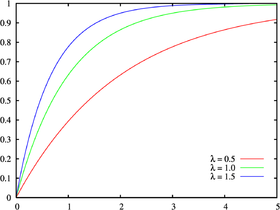
\includegraphics[width=0.6\textwidth]{./Images/Courbes_loi_exp}\\[0.9 cm]

	% Author and supervisor
	\begin{minipage}{0.4\textwidth}
		\begin{flushleft} \large
			\emph{Auteurs:}\\
			Thibaut \textsc{André-Gallis} \\
			{\small\href{mailto:thibaut.andregallis@insa-rouen.fr}{thibaut.andregallis@insa-rouen.fr}} \\
			Kévin \textsc{Gatel} \\
			{\small\href{mailto:kevin.gatel@insa-rouen.fr}{kevin.gatel@insa-				rouen.fr}}
		\end{flushleft}
	\end{minipage}
	\begin{minipage}{0.4\textwidth}
		\begin{flushright} \large
			\emph{Enseignant:} \\
			Julien \textsc{Saunier} \\
			{\small\href{mailto:julien.saunier@insa-rouen.fr}								{julien.saunier@insa-rouen.fr}}
		\end{flushright}
	\end{minipage}
	\vspace*{\stretch{1}}

	\vfill
	{\large 27 Novembre 2020}
\end{center}
\end{titlepage}

\tableofcontents

%\listoffigures

\renewcommand{\chaptername}{}
\chapter*{Introduction}
%\label{chapter:Introduction}
\addcontentsline{toc}{chapter}{Introduction}

La loi exponentielle modélise la durée de vie d'un phénomène sans mémoire ou sans vieillissement. En d'autres termes la probabilité que le phénomène dure au moins $h+t$ heures sachant qu'il a déjà duré $t$ heures sera la même que la probabilité de durer $h$ heures à partir de sa mise en fonction initiale. Elle peut notamment modéliser la vie des circuits électriques, résoudre des problématiques de durée de vie en général.\\

Dans ce projet nous allons nous intéresser à comment simuler et modéliser une loi exponentielle de paramètre $\lambda$. Dans un premier temps nous allons démontrer qu'il est possible d'obtenir une loi exponentielle en partant d'une loi uniforme, ensuite nous allons démontrer que prendre une loi uniforme $U$ ou bien $1-U$ ne change rien pour en obtenir une, enfin nous allons créer une loi exponentielle à expérimentalement à partir d'une loi uniforme à afin d'appliquer directement les parties précédentes.

\chapter{G(U) $\sim$ $\varepsilon(\lambda)$}

Soit $U$ une loi uniforme sur [0,1].

On a :

$$\mathbb{P}(U\leq t)=F_{U}(t)=\begin{cases}
0 & \text{si \ensuremath{t<0} }\\
\frac{t-0}{1-0}=t & \text{si \ensuremath{t}}\in[0,1]\\
1 & \text{si \ensuremath{t>1}}
\end{cases}$$

Soit $\lambda>0$ et $G$ une fonction telle que : \\

$$\begin{array}{ccccc}
	G & : & [0,1] & \longrightarrow & \mathbb{R}^{+} \\
	& & u & \longmapsto & \frac{-1}{\lambda}\ln(1-u) \\
\end{array}$$

Alors : \\
$$\mathbb{P}(G(U)<t)=\mathbb{P}(\frac{-1}{\lambda}\ln(1-U)<t)=\mathbb{P}(\ln(1-U)>-\lambda t)=\mathbb{P}(1-U>e^{-\lambda t})$$
Or :
$$\mathbb{P}(1-U>e^{-\lambda t})=\mathbb{P}(U<1-e^{-\lambda t})=F_{U}(1-e^{-\lambda t})=\begin{cases}
0 & \text{si \ensuremath{1-e^{-\lambda t}<0}}\\
1-e^{-\lambda t} & \text{si \ensuremath{\ensuremath{1}-}\ensuremath{e^{-\lambda t}}}\in[0,1]\\
1 & \text{si \ensuremath{1-e^{-\lambda t}>1}}
\end{cases}$$

On a :
$$\begin{array}{ccl}
	1-e^{-\lambda t}<0 & \iff & e^{-\lambda t}>1 \\
					   & \iff & \underbrace{-\lambda}_{<0}t>0 \\
					   & \iff & t<0 \\
\end{array}$$\\

Ensuite :
$$\begin{array}{ccl}
	1-e^{-\lambda t}\in[0,1] & \iff & 0\leq1-e^{-\lambda t}\leq1 \\
					   & \iff & e^{-\lambda t}\leq1 \\
					   & \iff & \underbrace{-\lambda}_{<0}t\leq0 \\
					   & \iff & t\geq0 \\
\end{array}$$\\

Enfin :
$$\begin{array}{ccl}
	1-e^{-\lambda t}>1 & \iff & e^{-\lambda t}<0 \\
	& \iff & t\in\emptyset \\
  \end{array}$$\\
  
Ainsi :
$$\mathbb{P}(G(U)<t)=\begin{cases}
0 & \text{si \ensuremath{t<0}}\\
1-e^{-\lambda t} & \text{si }t\geq0
\end{cases}$$\\

D'où $G(U) \sim \varepsilon(\lambda)$.
 
\chapter{G(U) $\sim$ G(1-U) $\sim$ $\varepsilon(\lambda)$}




\end{document}
